\documentclass{article}
\usepackage{amsmath, amssymb , amsthm, graphicx}

\begin{document}

\section*{Problem 1}

~

\begin{proof}
~
    \begin{enumerate}
        \item By Eudoxus’s definition of equality of ratios, $a:b=c:d \iff (\forall m,n\in\mathbb{Z}, ma>=<nb\iff mc>=<nd)$
        \item $\forall m,n\in\mathbb{Z}, ma>=<nc\iff mab>=<ncb\iff (mb)a>=<(nc)b$
        \item So by transitivity of $\iff:a:b=c:d \iff (\forall m,n\in\mathbb{Z}, (mb)a>=<(nc)b\iff (mb)c>=<(nc)d \iff (mc)b>=<(nc)d) \iff mb>=<md)$
        \item So by transitivity of $\iff:a:b=c:d \iff (\forall m,n\in\mathbb{Z},ma>=<nc\iff mb>=<md)$
        \item By Eudoxus’s definition of equality of ratios, $a:c=b:d \iff (\forall m,n\in\mathbb{Z},ma>=<nc\iff mb>=<md)$
        \item By transitivity of $\iff:a:b=c:d \iff a:c=b:d$
    \end{enumerate}
\end{proof}

\newpage

\section*{Problem 2}

~

\begin{proof}
    ~
    \begin{enumerate}
        \item Connect every vertex with the center of the circle, so there are $n$ congruent triangles ($SSS$). 
        \item The central angle is $\frac{2\pi}{n}$.
        \item Draw a perpendicular line from the center to the other side, since it is an isosceles triangle, the line also bisects the central angle and the side.
        \item Since the perpendicular line is also the radius, half of the side is $r\tan\frac{\pi}{n}$, the side is $2r\tan\frac{\pi}{n}$.
        \item The area of the triangle is $r^2\tan\frac{\pi}{n}$.
        \item The polygon has $n$ congruent triangles, so the area of the polygon is $nr^2\tan\frac{\pi}{n}$.
        \item $\lim_{n\to\infty}(nr^2\tan\frac{\pi}{n})=nr^2\lim_{n\to\infty}(\tan\frac{\pi}{n})=nr^2\frac{\pi}{n}=\pi r^2$
        \item As $n$ tends to infinity, a regular polygon becomes a circle, so the area of a circle is $\pi r^2$.
    \end{enumerate}
\end{proof}

\newpage

\section*{Problem 3}

~

\subsection*{a}

~

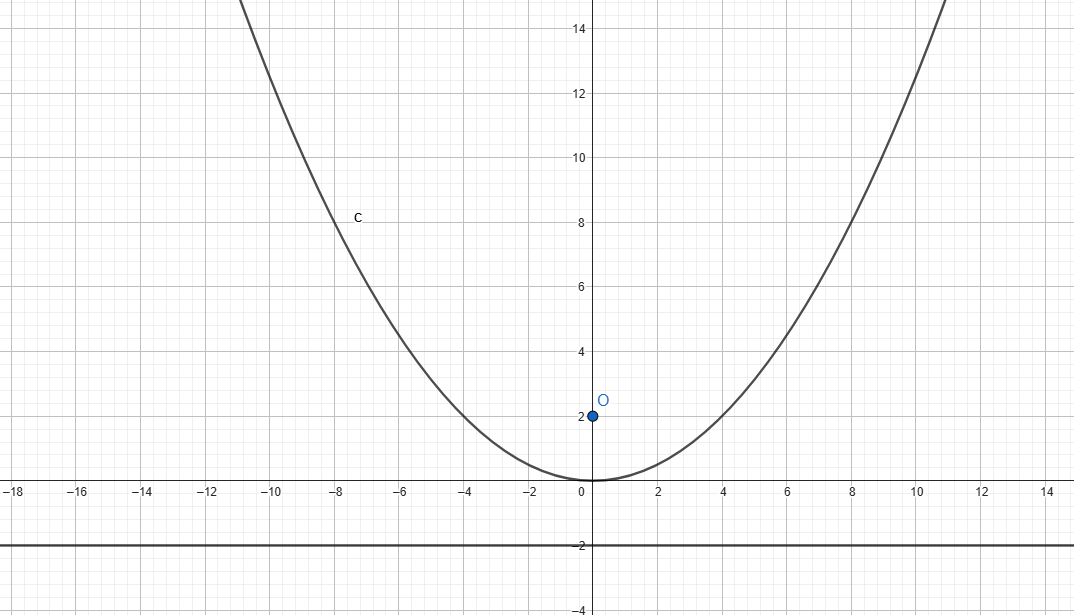
\includegraphics[scale=0.3]{HW_0307/3a.png}

~
\begin{align*}
        &O\text{ is the focus}:(0,\frac{p}{2})\\
        &l\text{ is the directrix}: y=\frac-{p}{2}\\
        &D_{OP}=D_{lP}\\
        &\sqrt{x^2+(y-\frac{p}{2})^2}=y+\frac{p}{2}\\
        &x^2+(y-\frac{p}{2})^2=(y+\frac{p}{2})^2\\
        &x^2=2yp\\
\end{align*}

~

\subsection*{b}

~

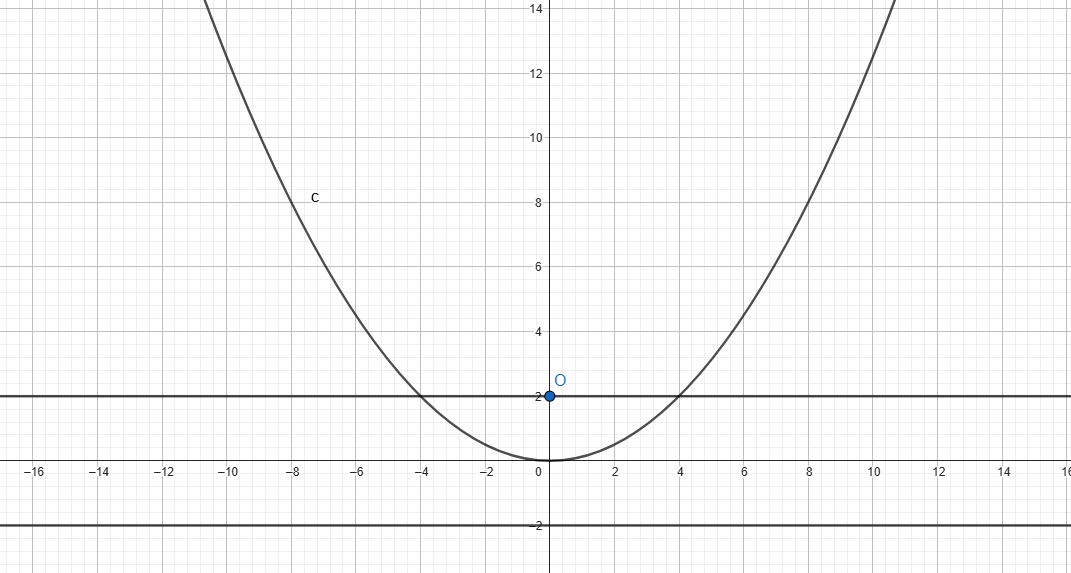
\includegraphics[scale=0.3]{HW_0307/3b.png}

~

\begin{align*}
    &\ell :y=\frac{p}{2}\\
    &x^2=2\frac{p}{2}p\\
    &x^2=p^2\\
    &x=\pm p\\
    \Rightarrow&D=2p\\
\end{align*}

~

\subsection*{c}

~

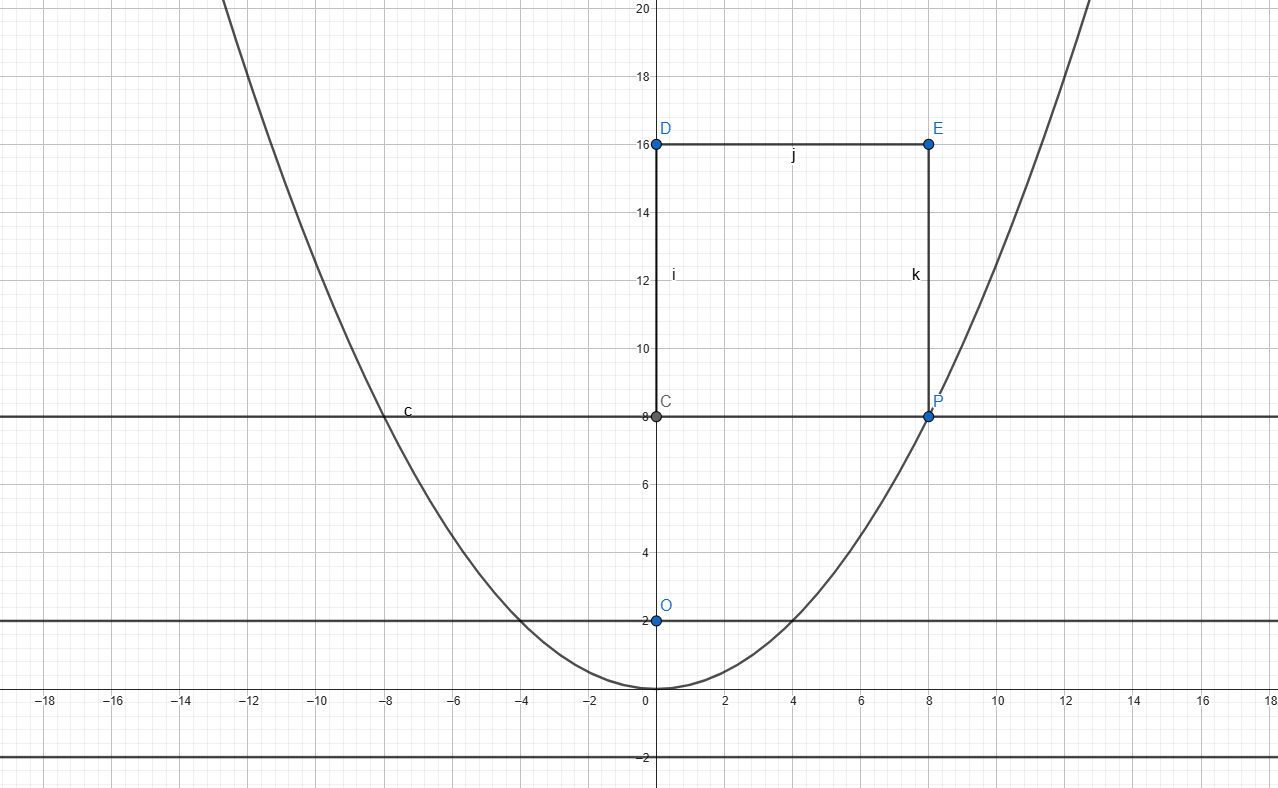
\includegraphics[scale=0.3]{HW_0307/3c.png}

~

\begin{align*}
    &\text{perpendicular is }y\text{-axis}\\
    \Rightarrow&D_P=|x|\\
    &A_{PCDE}=|x|^2=x^2\\
\end{align*}

~

\subsection*{d}

~

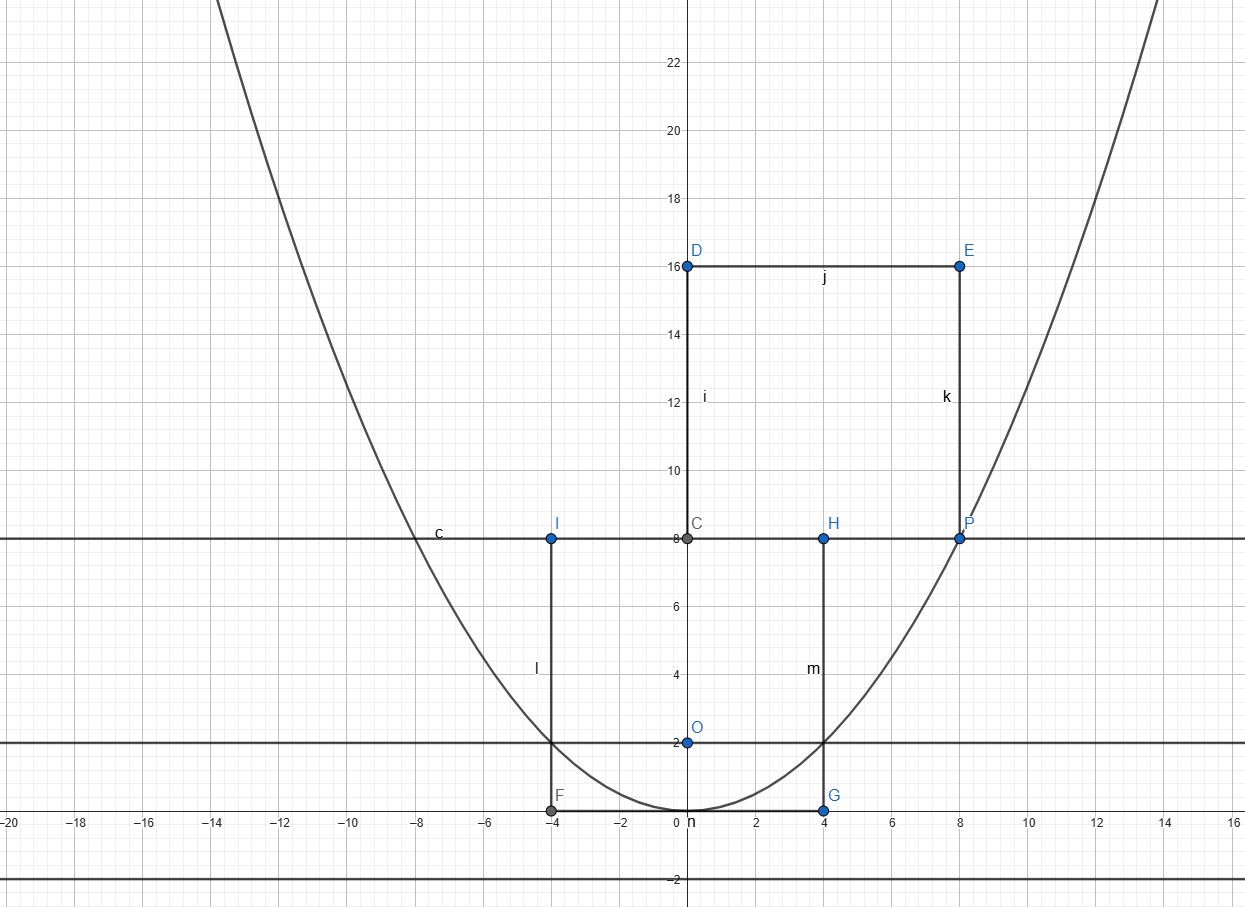
\includegraphics[scale=0.3]{HW_0307/3d.png}

~

\begin{align*}
    &D_\ell=2p\\
    &H=y\\
    \Rightarrow&A_{FGHI}=2py\\
    &x^2=2py\\
    \Rightarrow&A_{FGHI}=A_{PCDE}\\
\end{align*}

\newpage

\section*{Problem 4}

~

\begin{proof}
    ~
    \begin{enumerate}
        \item $y=x^2$, so $2p=1$, $p=\frac{1}{2}$, so focus is $(0,\frac{1}{2}p)=(0,\frac{1}{4})$
        \item Directrix is $y=-\frac{1}{4}$\\
        \item Suppose $A:(a,a^2)$, then tangent of $y=x^2$ at $A$ is $y-a^2=\frac{dy}{dx}(x-a)\implies y=2ax-a^2$
        \item Since perpendicular to directrix is vertical, the incoming angle is $\theta=\arctan(\frac{1}{2a})$.
        \item By reflection law, reflecting angle is also $\theta=\arctan(\frac{1}{2a})$.
        \item So the angle between the ray through focus and $y$-axis is $2\arctan(\frac{1}{2a})$
        \item $\tan(2\arctan(\dfrac{1}{2a}))=\dfrac{2\tan(\arctan(\dfrac{1}{2a}))}{1-{\tan^2(\arctan(\dfrac{1}{2a})})}=\dfrac{a}{a^2-\frac{1}{4}}$
        \item So the equation for reflecting ray is $y-a^2=\dfrac{a^2-\frac{1}{4}}{a}(x-a)$
        \item Substituting $y=\frac{1}{4},x=0$:
            \begin{enumerate}
                \item $LHS=\dfrac{1}{4}-a^2$
                \item $RHS=\dfrac{a^2-\frac{1}{4}}{a}\cdot (-a)=\frac{1}{4}-a^2$
                \item $LHS=RHS$
            \end{enumerate}
        \item The focus lands on the ray.
        \item All rays perpendicular to the directrix reflect through the focus.
    \end{enumerate}
\end{proof}

\newpage

\section*{Problem 5}

~
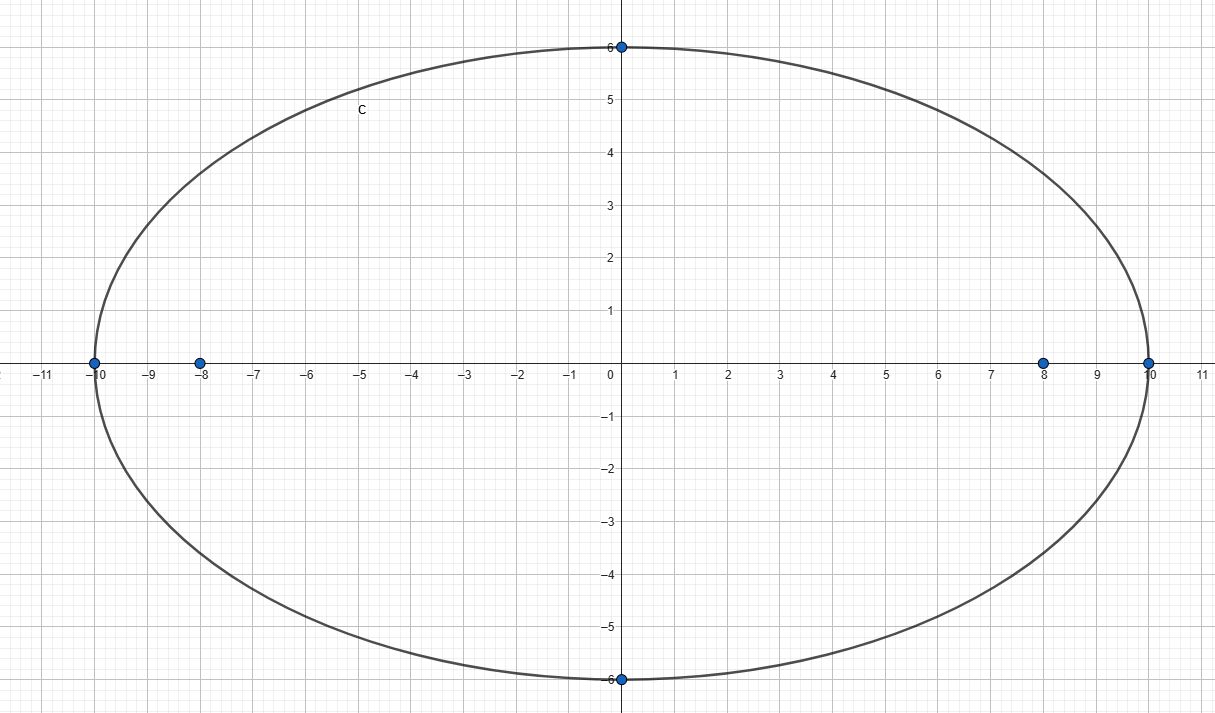
\includegraphics[scale=0.3]{HW_0307/5.png}

~

\subsection*{a}

~

\begin{enumerate}
    \item The sum of the distances from any point on the ellipse to the foci is $2a$.
    \item At $(0,b)$, the sum of the distances are $\sqrt{(b-0)^2+(0-c)^2}+\sqrt{(b-0)^2+(0+c)^2}=2\sqrt{b^2+c^2}$.
    \item $2\sqrt{b^2+c^2}=2a\implies a^2=b^2+c^2$
\end{enumerate}

~

\subsection*{b}

~

\begin{enumerate}
    \item Since the ellipse is symmetry, the two latus recta have the same length.
    \item Substitute $x=c$ into ellipse equation:
        \begin{enumerate}
            \item $\dfrac{x^2}{a^2}+\dfrac{y^2}{b^2}=1$
            \item $\dfrac{c^2}{a^2}+\dfrac{y^2}{b^2}=1$
        \end{enumerate}
    \item Substitute $c^2=a^2-b^2$:
        \begin{enumerate}
            \item $\dfrac{a^2-b^2}{a^2}+\dfrac{y^2}{b^2}=1$
            \item $\dfrac{y^2}{b^2}=\dfrac{b^2}{a^2}$
            \item $y=\pm\dfrac{b^2}{a}$
        \end{enumerate}
    \item $\ell=\dfrac{b^2}{a}-(-\dfrac{b^2}{a})=\dfrac{2b^2}{a}$
\end{enumerate}

~

\subsection*{c}

~

\begin{proof}
    ~
    \begin{enumerate}
    \item WLOG: Suppose $x\in[0,a)$ so that the distance to the nearest vertex is $a-x$, in $x<0$ it is $a+x$
    \item From ellipse equation:
        \begin{enumerate}
            \item $\dfrac{x^2}{a^2}+\dfrac{y^2}{b^2}=1$
            \item $y^2=b^2(1-\dfrac{x^2}{a^2})$
        \end{enumerate}
    \item $\ell(a-x)=\dfrac{2b^2(a-x)}{a}$
    \item $\dfrac{\ell(a-x)}{y^2}$:
        \begin{align*}
            &\frac{\ell(a-x)}{y^2}\\
            =&\frac{\frac{2b^2(a-x)}{a}}{b^2(1-\frac{x^2}{a^2})}\\
            =&\frac{2a(a-x)}{a^2-x^2}\\
            =&\frac{2a}{a+x}\\
        \end{align*}
    \item $x\in[0,a)$, so $\dfrac{2a}{a+x}>1$
    \item So $y^2<\ell(a-x)$
\end{enumerate}
\end{proof}
\end{document}